\chapter{Java para Web}
\epigraph{``\textit{Uma longa viagem começa com um único passo.}''.}{Lao-Tsé}

\lettrine[lines=4, lhang=0.1, lraise=0, loversize=0.2, findent=0.1em]{\textcolor{corAzulTema}{N}}{ESTE} Capítulo teremos como objetivos entender o funcionamento e a arquitetura de aplicações Web desenvolvidas em Java, entender o funcionamento dos Servlets e dos JSPs e aprender a configurar e a utilizar a \textit{Integrated Development Environment} (IDE) Apache NetBeans para o apoio ao desenvolvimento de aplicações Web em Java.


\section{Introdução}

Para que você seja capaz de construir aplicações Web, primeiramente é preciso conhecer como esse serviço é estruturado. A \textit{World Wide Web} (WWW), ou simplesmente Web, é um serviço executado em diversos computadores interligados em uma rede mundial, sendo que em alguns desses computadores são executados programas chamados de \textbf{servidores}, enquanto na maioria dos outros são executados programas chamados \textbf{clientes}, que se comunicam com os servidores, estes por sua vez servem recursos para estes clientes. Na Figura~\ref{fig:cap01ClienteServidor} é ilustrado um recorte desta rede mundial.

\FloatBarrier
\begin{figure}[!htbp]
    \centering
    \caption{Recorte da estrutura da WWW}
    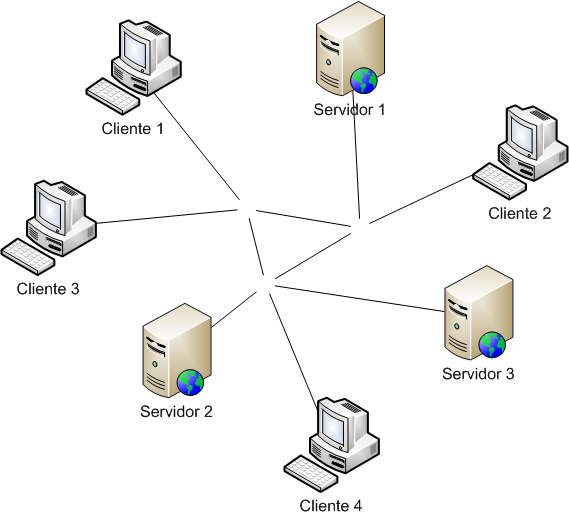
\includegraphics[scale=0.6]{imagens/cap01ClienteServidor}
    \\\textbf{Fonte:} Elaborada pelo autor
    \label{fig:cap01ClienteServidor}
\end{figure}
\FloatBarrier

Perceba que no recorte apresentado na Figura~\ref{fig:cap01ClienteServidor} são mostrados sete computadores, sendo que quatro deles atuam como clientes e os outros três como servidores. É importante entender que o que faz um computador ser cliente ou servidor é o tipo de programa que está sendo usado/executado. No nosso exemplo, as máquinas que atuam como servidores executam um programa denominado Servidor Web, que tem a capacidade de servir (disponibilizar) aos outros computadores da rede, recursos que fazem parte de uma aplicação Web, por exemplo, arquivos \textit{Hypertext Markup Language} (HTML), imagens em diversos formatos, arquivos de estilo, arquivos de \textit{script} etc. Os clientes, por sua vez, são, na maioria das vezes, os conhecidos navegadores Web, ou \textit{browsers}, que usamos no nosso dia a dia para acessar a Web e navegar em diversos \textit{sites}.

Da mesma forma que existem diversos navegadores, existem também alguns Servidores Web, sendo o Apache o mais famoso e o mais utilizado. Como já foi dito, um Servidor Web tem a função de servir recursos requisitados pelos clientes. Vamos aprender como isso funciona. Veja a Figura~\ref{fig:cap01RequestResponse}.

\FloatBarrier
\begin{figure}[!htbp]
    \centering
    \caption{Processo de requisição e resposta (\textit{request}/\textit{response})}
    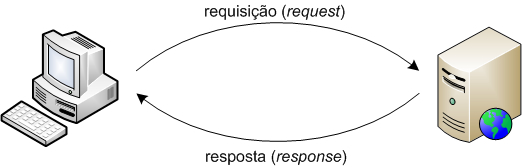
\includegraphics[scale=0.6]{imagens/cap01RequestResponse}
    \\\textbf{Fonte:} Elaborada pelo autor
    \label{fig:cap01RequestResponse}
\end{figure}
\FloatBarrier

Na Figura~\ref{fig:cap01RequestResponse} é mostrado o processo de requisição e resposta. Nesse processo, o cliente à esquerda (navegador), envia uma requisição a um recurso contido no Servidor Web (à direita) através de uma \textit{Uniform Resource Locator} (URL), sendo que nessa requisição, o cliente especifica o protocolo a ser usado, o endereço do servidor e o caminho para o recurso. Assim, uma URL tem a seguinte forma:

\begin{center}
    \textbf{\texttt{protocolo://máquina/caminho\_do\_recurso}}
\end{center}

\begin{itemize}
    
    \item Onde:
    
    \begin{itemize}
    
        \item \textbf{protocolo:} é a parte da URL que diz ao servidor qual o protocolo a ser utilizado. Quando acessamos páginas Web, por padrão, o protocolo utilizado é o \textit{Hypertext Transfer Protocol} (HTTP);
        
        \item \textbf{máquina:} é o nome ou o endereço codificado pelo \textit{Internet Protocol} (IP) da máquina que está executando o Servidor Web;
        
        \item \textbf{caminho\_do\_recurso:} é o caminho completo do recurso desejado que é disponibilizado pelo servidor.
        
    \end{itemize}
    
\end{itemize}

Confuso? Nem tanto. Vamos a um exemplo! Imagine a seguinte situação: Queremos acessar o site do IFSP. Para isso, abra o seu navegador e preencha o campo endereço com \texttt{http://www.ifsp.edu.br/} e tecle \texttt{<ENTER>}. Fazendo isso, o navegador envia uma requisição através de uma URL, usando o protocolo HTTP para a máquina \texttt{www.ifsp.edu.br}, que por sua vez retorna ao navegador uma página HTML que representa aquele endereço. 

Perceba que não especificamos o caminho do recurso! Isso não foi necessário, pois os Servidores Web são normalmente configurados para ter um comportamento padrão para responder às requisições onde só seja especificado o nome da máquina e esse comportamento padrão é direcionar para o recurso \texttt{index.html}, que é um arquivo HTML. Portanto, usar o endereço \texttt{http://www.ifsp.edu.br/} é o mesmo que usar o endereço \texttt{http://www.ifsp.edu.br/index.html}. Faça um teste! Coloque o endereço com o caminho do recurso (\texttt{index.html}) e tecle \texttt{<ENTER>}. O que aconteceu? A mesma página foi exibida não foi? Ótimo!

Vamos fazer mais um teste? Preencha novamente a barra de endereços no seu navegador com o endereço \texttt{http://j.i.uol.com.br/galerias/psp/patapon201.jpg} e tecle \texttt{<ENTER>}. Deve ter aparecido uma imagem de um jogo não foi? Vamos analisar a URL: usamos o protocolo HTTP, para pedir para o Servidor Web que está executando na máquina \texttt{j.i.uol.com.br} o recurso \texttt{patapon201.jpg}, que está armazenado no caminho \texttt{/galerias/psp/}. Este processo é ilustrado na Figura~\ref{fig:cap01ExemploRequestResponse}.

\FloatBarrier
\begin{figure}[!htbp]
    \centering
    \caption{Exemplo do processo de requisição e resposta a um recurso}
    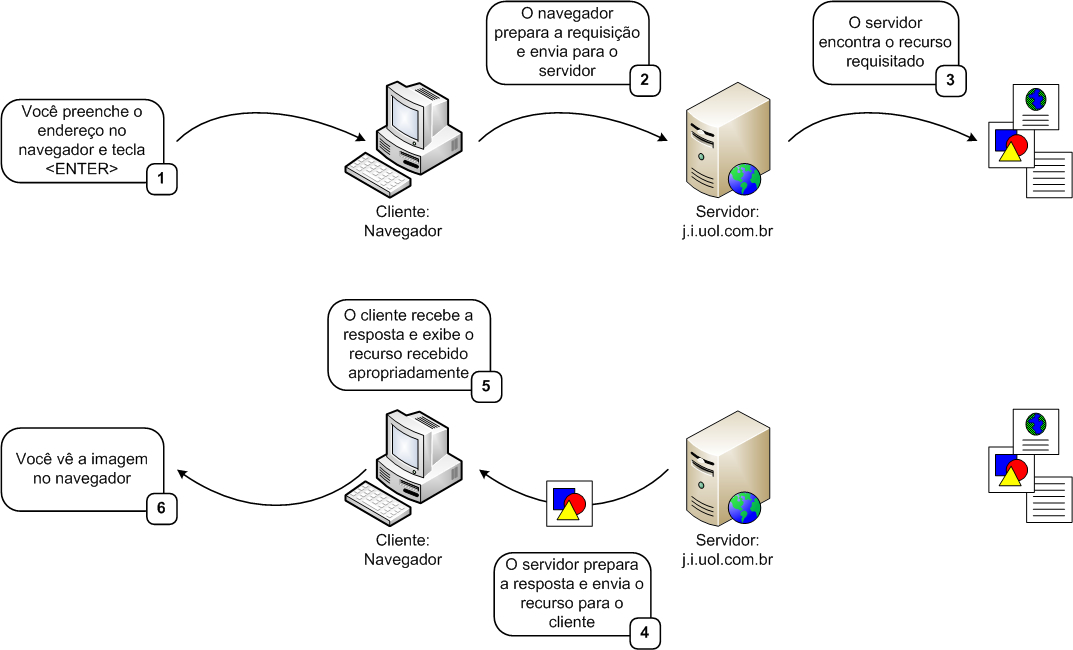
\includegraphics[scale=0.38]{imagens/cap01ExemploRequestResponse}
    \\\textbf{Fonte:} Elaborada pelo autor
    \label{fig:cap01ExemploRequestResponse}
\end{figure}
\FloatBarrier

Perceba que os passos 1, 2 e 3 da Figura~\ref{fig:cap01ExemploRequestResponse} representam o processo de requisição, enquanto os passos 4, 5 e 6 representam o processo de resposta. Note também que ao clicar em qualquer \textit{link}\footnote{O termo \textit{link} será usado para designar os \textit{hyperlinks} dos arquivos HTML} em uma página, todo esse processo é executado pelo navegador.

Muito bem! Agora que você já sabe como funciona o processo de requisição e resposta entre um navegador e um Servidor Web, podemos prosseguir com nossos estudos, agora focando em como a linguagem e a plataforma Java são utilizadas para trabalhar com aplicações Web.


\section{\textit{Container} de Servlets e Servidores de Aplicações}

Na seção anterior você aprendeu algumas coisas novas\footnote{Provavelmente você já sabia disso!}, mas onde que a linguagem Java se encaixa nisso tudo? Quando criamos aplicações Web, além de termos páginas com código HTML e outros recursos como imagens, por exemplo, precisamos ter também componentes que processem informações que queremos que nossa aplicação manipule. Imagine que você vai fazer \textit{login} na sua rede social favorita (Facebook, Instagram etc.). Você preenche um campo com seu nome de usuário, sua senha e clica no botão para acessar o sistema e então eu lhe pergunto: O que acontece? Quem que vai validar seu usuário e sua senha? Como você deve saber uma página HTML não consegue fazer isso não é mesmo? Veja a tela de \textit{login} do Facebook na Figura~\ref{fig:cap01LoginFacebook}.

\FloatBarrier
\begin{figure}[!htbp]
    \centering
    \caption{Tela de login da rede social Facebook}
    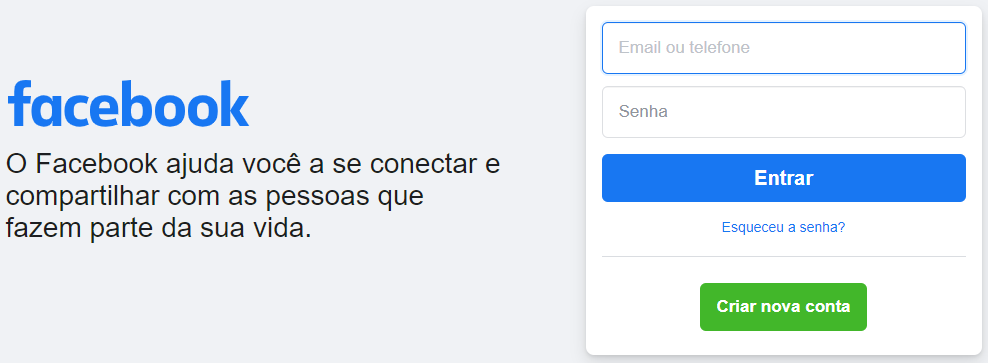
\includegraphics[scale=0.38]{imagens/cap01LoginFacebook}
    \\\textbf{Fonte:} \textit{Print screen} de \url{http://www.facebook.com}, acessado em 18/06/2021
    \label{fig:cap01LoginFacebook}
\end{figure}
\FloatBarrier

O responsável em processar os dados enviados é um componente de software que é executado no servidor em que a aplicação Web está implantada. Se a aplicação é feita em PHP, um script PHP vai fazer essa validação e retornar algum resultado com base no que foi verificado. Se a aplicação for feita em ASP.NET, Node.js etc. acontece o mesmo, ou seja, algum componente vai tratar a requisição -que enviou o usuário e a senha- e vai validá-la. Em Java é a mesma coisa!

Para que possamos utilizar código Java em nossas aplicações Web, recorremos a alguns componentes que podem ser criados dentro delas, sendo que o tipo principal desses componentes é o Servlet. Você se lembra do nosso exemplo do Facebook? Os desenvolvedores do Facebook, se usassem Java, poderiam ter criado um Servlet para receber os dados do formulário de \textit{login}, processá-los e retornar alguma resposta para o cliente, que no caso, normalmente é um navegador.

Muito bem. Sabemos então que se usarmos Java para desenvolver nossas aplicações Web, os componentes que são capazes de processar dados nas nossas aplicações e retornar resultados são os Servlets. Os Servlets são executados e gerenciados pelos \textit{Containers} de Servlets, que funcionam como um Servidor Web simples, mas com alguns ``poderes'' a mais. Esses \textit{Containers} também podem ser componentes de infraestruturas ainda mais robustas, que no caso são os Servidores de Aplicações. Um Servidor de Aplicações é como se fosse um \textit{Container} de Servlets com anabolizantes, pois além de implementar toda a especificação dos Servlets e as especificações ligadas a eles, esse tipo de servidor também implementa uma série de outras especificações da plataforma Jakarta EE (\textit{Enterprise Edition})\footnote{\url{https://jakarta.ee/}}, atigamente denominada Java EE, que fogem do propósito deste livro.

Da mesma forma que existem navegadores e Servidores Web diferentes, adivinhe só, existem também Servidores de Aplicações e \textit{Containers} de Servlets diferentes! Iremos utilizar na nossa disciplina a implementação de referência das especificações do Jakarta EE 8, que é feita pelo Servidor de Aplicações Eclipse Glassfish 5.1. Trabalharemos com essa versão, que mesmo não sendo a mais recente, será a ideal para o que precisaremos fazer e que tem um melhor suporte no NetBeans. Quando estamos no mundo ``Java para Web'', várias dúvidas surgem o tempo todo, visto que existe uma infinidade de termos diferentes e que normalmente causam confusão, além de existir um ecossistema absurdamente vasto. Na próxima seção vamos aprender mais alguns detalhes teóricos e na última seção vamos realizar algumas atividades!


\section{Servlets e JSPs}

Um carro serve para dirigir. Uma televisão para assistir. Uma sandália para andar. Cada um tem suas características e vão evoluindo com o tempo. Há muito tempo atrás, quando foi inventada a televisão, a imagem que era gerada não era muito boa e era em preto e branco. Foram passando os anos e a indústria foi evoluindo o equipamento. Primeiro a imagem melhorou, depois colocaram cores, depois foram criando telas cada vez maiores, mais finas, com maior resolução, inventaram outras formas de emitir imagens, gastar menos energia elétrica e assim por diante. E daí?

Tudo evolui. O que não evolui é descartado e/ou substituído. A primeira especificação dos Servlets foi lançada em 1997 e de lá para cá, a especificação foi evoluindo, permitindo que os Servlets se tornassem componentes mais versáteis e mais fáceis de utilizar. Na versão 5.1 do Eclipse Glassfish (perfil \textit{Web}) que implementa as especificações do Jakarta EE 8 (perfil \textit{Web}), é implementada a especificação 4.0 dos Servlets, a especificação 2.3 das JSPs (JavaServer Pages), entre outras.

Já aprendemos que os Servlets são componentes de uma aplicação Web feita em Java e que têm a capacidade de processar dados enviados a eles e gerar respostas. Um Servlet pode gerar como resposta o código HTML de uma página, entretanto essa abordagem era utilizada nas versões mais antigas dos Servlets e é totalmente desencorajada hoje em dia. Como eu disse agora a pouco, tudo evolui. Para que os desenvolvedores não precisassem mais gerar código HTML dentro do código Java de um Servlet, foram inventadas as páginas JSP. Uma página JSP é um arquivo que pode conter –e geralmente contém– código HTML e que pode interagir diretamente com algumas funcionalidades de uma aplicação Web.

A rigor, um JSP é processado pelo Servidor de Aplicações e todo o seu conteúdo é traduzido em um Servlet, que por sua vez é compilado e executado pelo Servidor. Todo esse processo é executado nos bastidores, então não precisamos nos preocupar com esses detalhes, mas é sempre bom saber um pouquinho como as coisas funcionam não é mesmo?

Por causa desse comportamento de tradução das JSPs para Servlets, nós podemos inserir código Java dentro das JSPs, mas novamente não iremos usar essa abordagem, muito menos irei ensinar como fazer, visto que da mesma forma que gerar HTML dentro de um Servlet manualmente é desencorajado, essa abordagem de inserir código Java dentro das JSPs também não deve ser utilizada. Uma JSP deve ser usada para exibir dados, não para processá-los diretamente usando código Java. Note que não estou dizendo que não iremos manipular dados dentro das JSPs, mas sim que existem formas seguras e corretas para fazer isso. Aprenderemos esses detalhes só no Capítulo 3, pois até lá, já teremos aprendido outros detalhes que ainda não foram apresentados.


\section{Preparação do Ambiente de Desenvolvimento}

Nesta seção você aprenderá a instalar e configurar a IDE Apache NetBeans e o Servidor de Aplicações Eclipse Glassfish 5.1 (perfil \textit{Web}).


\subsection{Apache NetBeans}

Você conhece a linguagem Java, aprendeu a teoria e a prática da programação orientada a objetos e provavelmente usou a IDE Apache NetBeans para escrever seus códigos. Neste livro trabalharemos com a versão 12 desta IDE e nos passos abaixo é explicado como deve ser feito o \textit{download} e a instalação da mesma. Esses passos podem ser pulados caso você já tenha a ferramenta instalada em seu computador.

\begin{enumerate}

    \item Acesse o endereço: \url{http://netbeans.org/downloads/}
    
    \item Haverá várias opções de download. Procure pela maior, especificada como ``Tudo''. É a da última coluna. Tem cerca de 319MB. Coloque o arquivo para baixar e vá tomar um café. Se tiver dúvida, dê uma olhada na Figura 1.5. Note que durante o desenvolvimento deste livro, a versão mais atual do NetBeans era a 6.9.1. Você pode baixar a mais recente caso esteja disponível.
    
    Figura 1.5: Baixando o NetBeans completo (\url{http://netbeans.org/downloads/})
    Fonte: Print screen, \url{http://netbeans.org/downloads/}
    
    \item Baixou? Execute o instalador. Logo no primeiro passo, clique no botão ``Personalizar...'' (canto inferior esquerdo) para personalizar a instalação. Como iremos utilizar o Tomcat como Container de Servlets, selecione-o para que ele seja instalado. Na Figura 1.6, estão marcados os componentes que você OBRIGATORIAMENTE precisa instalar (IDE de base, Java SE, Java Web e EE, Recursos sob demanda, Apache Tomcat 6.0). Se quiser instalar outros componentes, fique à vontade.
    
    Figura 1.6: Personalização da instalação do NetBeans
    Fonte: Print screen, NetBeans IDE 6.9.1
    
    \item Clique no botão ``OK'' do diálogo de personalização e vá clicando em ``Próximo'' até que a instalação termine. Ao terminar, feche o instalador. Um ícone do NetBeans vai ter sido criado na sua área de trabalho. Com isso terminamos nosso tutorial super-rápido de instalação do NetBeans.
    
\end{enumerate}

Com o NetBeans instalado, abra-o. Caso o esteja executando pela primeira vez, uma página de boas-vindas será exibida. Você pode fechá-la se quiser, além de marcar para que não seja exibida novamente. Vamos criar então nosso primeiro projeto Web!

\begin{itemize}

    \item \textbf{Passo 1:} Clique no meu ``Arquivo'' e depois em ``Novo Projeto''. Fazendo isso, o assistente para criação de projetos será aberto. Na lista de categorias, escolha ``Java Web'' e na lista de tipos de projeto, escolha ``Aplicação Web'' e clique no botão ``Próximo''. 
    
    \item \textbf{Passo 2:} Preencha o campo ``Nome do projeto'' com ``OlaMundoWeb'' (sem acentos e sem as aspas e tudo junto). Em ``Local do projeto'', defina o diretório onde o projeto será salvo. Deixe a opção ``Usar pasta dedicada para armazenar bibliotecas'' desmarcada e marque a opção ``Configurar como projeto principal''. Clique no botão ``Próximo''.
    
    \item \textbf{Passo 3:} Na opção ``Servidor'' escolha o Apache Tomcat 6.0.xx. Em ``Versão do Java EE'' escolha ``Java EE 5''. Em ``Caminho do Contexto'' deixe o valor padrão (/OlaMundoWeb), que é o mesmo nome que demos ao nosso projeto. Clique em ``Próximo''.
    
    \item \textbf{Passo 4:} Neste passo, o assistente pergunta quais frameworks nós queremos inserir no nosso projeto. Nós não vamos usar nenhum, então basta clicar em ``Finalizar''. Fazendo isso, o novo projeto será criado e será aberto no NetBeans, sendo que por padrão será criado um arquivo JSP (index.jsp) que será a página arquivo inicial da nossa aplicação.
    
\end{itemize}

\begin{saibaMais}
    Um framework é um conjunto de classes que são usadas para executar uma determinada tarefa específica.
\end{saibaMais}

Muito bem, criamos nosso primeiro projeto. Vamos executá-lo para ver o que acontece? Na barra de ferramentas do NetBeans tem um botão com uma seta verde, igual a um botão de ``play'' de um CD Player. Quando você clicar nesse botão, você vai ver que várias mensagens começarão a aparecer na janela de saída do NetBeans. Essas mensagens irão mostrar para nós o que está acontecendo no momento, como a inicialização do Tomcat, por exemplo. O que está esperando? Clique lá no ``play''. Assim que tudo estiver pronto, será aberta uma janela do seu navegador, onde será mostrado o conteúdo do index.jsp, que no nosso caso será uma página com um ``Hello World!'' escrito.

Muito bem! Temos nossa primeira aplicação rodando no Tomcat! Fácil não é mesmo? Por enquanto não vamos nos preocupar com a estrutura do projeto, iremos aprender os detalhes aos poucos. Vamos colocar um pouco de código HTML no nosso index.jsp? Ele deve estar aberto no NetBeans. Se não estiver, procure o arquivo index.jsp na pasta ``Páginas Web'' do seu projeto e clique duas vezes no arquivo para abri-lo no editor. Vamos mudar o título, escrever ``Olá Mundo!'' no lugar de ``Hello World!'' e inserir um link para a página do IFSP. Veja na Listagem 1.1 como ficou o meu código.

Listagem 1.1: Código do arquivo index.jsp
\htmlCode{Teste}{projetos/capitulo01/OlaMundoWeb/web/index.html}
Fonte: do autor

Salve o arquivo depois de editá-lo. Se o navegador ainda estiver aberto no index.jsp, volte a ele e aperte a tecla F5 do seu teclado para mandar o navegador atualizar a página. Se não estiver, dê o ``play'' no projeto de novo. Você vai ver que a página vai exibir as alterações que fizemos. Teste o link para ver se está funcionando. A página deve ter ficado como mostrada na Figura 1.7.

Figura 1.7: Arquivo index.jsp em exibição
Fonte: Print screen, Windows 7

Uma JSP basicamente é um arquivo com código HTML que pode conter outros tipos de estruturas que vamos aprender no decorrer da disciplina. Por enquanto vamos ficar por aqui com as JSPs. Vamos testar os Servlets agora? Como primeiro exemplo, nós vamos criar um Servlet manualmente, enquanto os outros que vamos desenvolver durante o nosso curso serão feitos usando um assistente do NetBeans, mas essa forma fácil nós só vamos aprender a partir da Aula 2.

Aprenderemos como criar manualmente um Servlet, para que possamos aprender alguns detalhes importantes sobre o funcionamento de aplicações Web feitas em Java.

\begin{itemize}
    \item \textbf{Passo 1:} Na árvore que representa a estrutura do projeto, procure pela pasta ``Pacotes de código-fonte'' e expanda-a (clique no sinal de ``+'' à esquerda). Dentro dela haverá um pacote com o ícone cinza chamado ``<pacote padrão>''. Como vocês devem saber, é desencorajado que se trabalhe com pacotes padrão em Java, então vamos criar um pacote. Clique com o botão direito na pasta ``Pacotes de código-fonte'' e escolha ``Novo'', procure pela opção ``Pacote Java...'' e clique nela. Se esta opção não estiver sendo exibida, clique na opção ``Outro...'' (no final da lista), escolha ``Java'' em ``Categorias'', ``Pacote Java'' nos ``Tipos de Arquivos'' e clique em ``Próximo''. Preencha o campo ``Nome do pacote'' com ``olamundoweb'' (sem as aspas) e clique em ``Finalizar''. O pacote será criado.
    
    \item \textbf{Passo 2:} Repita o Passo 1, só que agora clicando com o botão direito no pacote que você criou e crie um pacote chamado ``servlets'' (sem as aspas). O nome do pacote deverá ser preenchido com ``olamundoweb.servlets''. Seu projeto agora terá um pacote chamado ``olamundoweb.servlets''.
    
    \item \textbf{Passo 3:} Clique com o botão direito no pacote ``olamundoweb.servlets'', escolha ``Novo'' e clique na opção ``Classe Java...''. Novamente, se não a encontrar, clique em ``Outro...'' e procure pela ``Classe Java'' (está na categoria ``Java'') e clique em ``Próximo''. Preencha o campo ``Nome da classe'' com ``OlaServlet'' (sem as aspas) e clique em ``Finalizar''. A classe será criada dentro do pacote especificado e será aberta no editor. Você vai ter algo como apresentado na Listagem 1.2.
    
    Listagem 1.2: Código da classe que será um Servlet
    Fonte: do autor
    
    \item \textbf{Passo 4:} Para que uma classe seja um Servlet, precisamos estender a classe HttpServlet, que está contida no pacote javax.servlet.http e então implementar os métodos HTTP que queremos que nosso Servlet trate. Não se preocupe, ainda vamos aprender sobre os métodos HTTP, então o importante, a saber, por enquanto, é que os métodos HTTP mais usados são o GET (doGet(...) de HttpServlet) e o POST (doPost(...) de HttpServlet). Então teremos que sobrescrever cada um desses métodos e ainda criaremos um terceiro que será invocado a partir dos outros dois. Confuso? Vamos ver como o código ficaria. Leia os comentários e copie o código para o seu editor!
    
    Listagem 1.3: Implementação do primeiro Servlet (parte 1)
    Fonte: do autor
    
    Listagem 1.4: Implementação do primeiro Servlet (parte 2)
    Fonte: do autor
    
\end{itemize}

Até agora criamos uma classe chamada OlaServlet, que estende a classe HttpServlet. Sobrescrevemos os métodos doGet e doPost herdados de HttpServlet que tratam respectivamente os métodos GET e POST do protocolo HTTP e criamos um terceiro método, chamado processRequest, que tem a mesma assinatura dos métodos doGet e doPost e que é invocado dentro deles. É no processRequest que iremos colocar o código que queremos executar, sendo que no nosso exemplo, estamos mandando imprimir na saída duas Strings: ``Olá Mundo!'' e ``Meu Primeiro Servlet!''. Ou seja, se chamarmos o Servlet usando o método GET, o método doGet será invocado e passará o controle para o método processRequest que irá imprimir as mensagens na saída. O mesmo acontece para o método POST.

Muito bem, você tem um Servlet totalmente funcional, mas ai você se pergunta: ``Como vou chamar esse Servlet através do navegador?''. Então eu respondo: ``Precisamos mapeá-lo e dar um endereço para ele.''. Ai você diz: ``Mas como?''. E eu respondo: ``Siga os passos a seguir.''

\begin{itemize}

    \item \textbf{Passo 1:} Na estrutura do projeto, procure por uma pasta chamada ``Arquivos de configuração''. Adivinhe o que tem dentro dela? Arquivos de configuração é claro! O que nos interessa é o web.xml, que vamos chamar de DI (Descritor de Implantação), do termo em inglês Deployment Descriptor, e que é um arquivo XML. É no DI que ficam especificadas as configurações na nossa aplicação e é nele que vamos fazer o tal mapeamento que falei. O que está esperando? Abra-o no editor. 
    
    \begin{saibaMais}
        Não sabe o que é XML? Dê uma olhada aqui: \url{http://pt.wikipedia.org/wiki/XML}
    \end{saibaMais}
    
    \item \textbf{Passo 2:} Para nos auxiliar, o NetBeans tem um editor gráfico para o DI. Ao abrir o web.xml, perceba que existem várias guias (Geral, Servlets, Filtros, Páginas, ..., XML). Adivinhe em qual iremos clicar. Clique na guia ``Servlets''. Ao clicar, procure pelo botão ``Adicionar elemento servlet...'' e clique nele. Um diálogo será aberto. Vamos preenchê-lo. Em ``Nome do Servlet'', vamos preencher com o mesmo nome da nossa classe Servlet, ou seja, ``OlaServlet'' (sem as aspas). Em ``Classe do servlet'' precisamos apontar para a nossa classe. Clique em procurar, expanda ``Pacotes de código-fonte'' até encontrar o arquivo ``OlaServlet.java''. Selecione-o e clique em ``Selecione o arquivo''. Deixe o campo ``Arquivo JSP'' em branco. Preencha descrição com ``meu primeiro servlet'' (sem as aspas) e por fim preencha o campo ``Padrão de URL'' com ``/ola'' (sem as aspas e não esqueça de inserir a barra). Veja a Figura 1.8. Clique em OK e salve o arquivo.
    
    Figura 1.8: Mapeando o primeiro Servlet
    Fonte: Print screen, NetBeans IDE 6.9.1
    
\end{itemize}

No Passo 2 fizemos o mapeamento para amarrar o Servlet ``OlaServlet'' a um padrão de URL. Lembra que preenchemos o campo ``Padrão URL'' com ``/ola''? Com isso, podemos agora acessar o OlaServlet a partir de uma URL, que no nosso caso é ``\url{http://localhost:8084/OlaMundoWeb/ola}'', ou seja, usamos o protocolo HTTP, para a máquina localhost (que é o endereço da nossa máquina), na porta 8084 (que é a porta que o Tomcat ouve), para acessar a aplicação chamada OlaMundoWeb (isso vem do contexto que criamos no Passo 3 da Seção 1.4, volte lá para dar uma olhadinha), para por fim acessar o recurso mapeado sob o nome de ``ola'' que no caso é o nosso Servlet. 

Sei que pode parecer um pouco confuso no começo, mas logo você vai pegar o jeito da coisa. Dê um ``Play'' no projeto de novo. O navegador vai abrir no endereço da aplicação novamente. Insira o ``ola'' (sem as aspas) no final da URL e tecle <ENTER>. O que aconteceu? Apareceu uma página em branco não foi? É claro, afinal, nosso Servlet não gera HTML, mas apenas imprime duas mensagens na saída padrão não é mesmo? Mas como podemos ver essas mensagens? Volte no NetBeans e procure, logo abaixo, uma aba chamada ``Saída'' (ela provavelmente vai estar selecionada). Dentro dela existem outras três abas: OlaMundoWeb (run) que deve estar selecionada e que é usada para mostrar o processo de compilação (na verdade não é só o processo de compilação que é exibido, mas sim todo o processo de construção do projeto) na nossa aplicação, Log Apache Tomcat 6.0.xx usada para mostrar os logs do nosso Container. Por fim, Apache Tomcat 6.0.xx, que exibe a saída padrão do Tomcat. Clique nessa última aba e veja o que está escrito lá embaixo. As duas mensagens que mandamos através do método println dentro do Servlet! Volte ao navegador e tecle <ENTER> novamente no endereço do Servlet. Volte no NetBeans. Mais duas mensagens! Fácil não é mesmo?

Para fechar a nossa primeira Aula, vamos voltar ao nosso DI (Descritor de Implantação). Abra novamente o web.xml e procure pela aba XML (a última). O web.xml é um arquivo XML que, como eu já disse, é responsável por manter todas as configurações da nossa aplicação. Apesar do NetBeans ter um editor gráfico para esse arquivo, sempre é bom entendermos, nem que seja um pouquinho, como as coisas funcionam nos bastidores. Ao clicar na aba XML será exibido o código do DI. Veja na Listagem 1.5.

Listagem 1.5: web.xml da aplicação
Fonte: do autor

O DI inicia com o preâmbulo padrão de um arquivo XML, <?xml...> e depois a primeira tag, chamada <web-app>, é utilizada. Essa é a tag principal do web.xml, que informa que esse arquivo é um DI. Dentro dela, temos primeiramente a tag <servlet>, que contém a descrição do Servlet, o nome dele e a classe Java correspondente. O que isso te lembra? Aquele diálogo que preenchemos no Passo 2 durante o mapeamento do Servlet (veja na Seção 1.4), não é? Após a tag <servlet>, onde o Servlet foi declarado, vem a tag <servlet-mapping> que é usada para mapear o Servlet. Veja que o nome definido dentro de <servlet-name> é o mesmo que está contido dentro da tag <servlet> e que dentro de <servlet-mapping> está declarado o mapeamento para ``/ola''.

A tag <session-config> não é importante agora. A tag <welcome-file-list> é usada para especificar a lista de arquivos que devem ser utilizados como ponto de partida quando acessamos nossa aplicação. Lembra que eu falei que em um Servidor Web nós podemos definir um arquivo padrão para ser aberto? No Tomcat, que é nosso Container, isso é feito dentro dessa tag. Olhe só quem está lá! O index.jsp, que é a página inicial que é mostrada quando acessamos nossa aplicação pelo endereço \url{http://localhost:8084/OlaMundoWeb}.

Por mais que nosso exemplo não tenha nenhuma utilidade aparente, ele foi importante para nós entendermos o funcionamento básico de uma aplicação Web feita em Java. Nas próximas aulas vamos colocar o que aprendemos em prática, além de aprender várias outras coisas, para criarmos um sistema de cadastro na forma de uma aplicação Web. Não se esqueça de praticar o que aprendemos até agora. 


\section{Resumo}

Nesta aula aprendemos o que é e como funciona uma aplicação Web em Java. Aprendemos a criar nosso primeiro projeto e alguns detalhes sobre a tecnologia que estamos utilizando. Executamos nossa aplicação e fizemos algumas modificações nela para vermos o que estava sendo feito. Criamos também – de forma manual – um Servlet, que como aprendemos é um dos componentes principais de uma aplicação Web em Java. Aprendemos também que existe um arquivo, denominado Descritor de Implantação – o web.xml – que descreve as características da nossa aplicação Web e onde fizemos o mapeamento do Servlet que criamos para uma URL válida dentro da nossa aplicação.


\section{Exercícios}

\begin{exercicioSemArquivo}{}{}{}
    O que é um Servidor Web?
\end{exercicioSemArquivo}

\begin{exercicioSemArquivo}{}{}{}
    Como são chamados os clientes que utilizamos para acessar aplicações servidas por um Servidor Web? Cite alguns exemplos.
\end{exercicioSemArquivo}

\begin{exercicioSemArquivo}{}{}{}
    Diferencie um Servidor Web de um Container de Servlets.
\end{exercicioSemArquivo}


\section{Projetos}

\begin{projetoSemArquivo}{}{}{}
    Crie um novo projeto Java Web no NetBeans, com o nome de ``MinhaPagina'', edite o index.jsp de modo a exibir seus dados pessoais, seus interesses, etc. Tente inserir uma imagem também. Dica: a imagem deve estar dentro do projeto do NetBeans. Pense se você entende o motivo pelo qual o arquivo index.jsp é mostrado por padrão quando você acessa sua página através da URL \url{HTTP://localhost:8084/MinhaPagina}.
\end{projetoSemArquivo}

\begin{projetoSemArquivo}{}{}{}
    Crie um novo projeto Java Web no NetBeans, com o nome de ``Contador''. Nesse projeto você deve criar um Servlet manualmente e dentro do método processRequest use um laço de repetição (for) para direcionar para a saída padrão os números de 1 a 30. Não se esqueça de mapear o Servlet no DI e de verificar se ao acessar a URL criada os números são exibidos.
\end{projetoSemArquivo}

\begin{projetoSemArquivo}{}{}{}
    Crie um novo projeto Java Web no NetBeans, com o nome de ``Fibonacci''. Nesse projeto, você deve criar um Servlet manualmente e dentro do método processRequest use um laço de repetição (for) para exibir os 30 primeiros termos da série de Fibonacci. Crie um método chamado fibonacci dentro do seu Servlet, sendo que este método deve receber como parâmetro um int e retornar um int. O int que é recebido como parâmetro é o número do termo desejado, enquanto o int que é retornado é o termo correspondente ao parâmetro que foi recebido. A série de Fibonacci é formada inicialmente pelos números 1 e 1, sendo que os próximos números da série são gerados a partir da soma dos dois números anteriores. Os sete primeiros termos da série de Fibonacci são:
    1, 1, 2, 3, 5, 8, 13, onde: 2 = 1 + 1, 3 = 1 + 2, 5 = 2 + 3, 8 = 3 + 5, 13 = 5 + 8
    Exemplos de chamadas da função fibonacci:
    fibonacci(2): retorna 1
    fibonacci(5): retorna 5
    fibonacci(7): retorna 13
\end{projetoSemArquivo}